\section{Algoritmos}

A continuación se detallan los códigos y los pasos que se siguieron para llevar a cabo los algoritmos planteados utilizando distintas técnicas de programación.

\subsection{Backtracking}

A continuación se detallan el código y los pasos que se siguieron para llevar a cabo el algoritmo planteado utilizando \textbf{\textit{Backtracking}}.

\subsubsection{Obtener las posibles soluciones}

Una vez se obtuvieron todos los subconjuntos de jugadores para cada partido:

\lstinputlisting[language=Python]{code/backtracking.py}

siendo:
\begin{itemize}
    \item $A$: Lista compuesta de $m$ listas, las cuales representan un conjunto de jugadores para jugar un partido.
    \item \texttt{jugadores}: Lista con un subconjunto de jugadores que representan una posible solución actual.
    \item \texttt{solucion}: Lista con todos los subconjuntos de jugadores que son soluciones.
    \item \texttt{n}: Número que indica sobre cuál de las $m$ listas estamos trabajando.
    \item \texttt{utilizados}: Diccionario cuyo par \textit{clave-valor} es \textit{jugador-n} donde $n$ representa la enésima-lista en la que fue utilizado el jugador.\footnote{Siendo $n$ el menor valor encontrado hasta el momento}
\end{itemize}

El algoritmo persigue la exploración de diversas soluciones mediante combinaciones, las cuales se ven restringidas mediante condiciones de poda. Este enfoque se implementa con el propósito de evitar la evaluación exhaustiva de todas las posibles combinaciones evitando que se convierta en un algoritmo de \textit{Fuerza Bruta}, optimizando así la eficiencia del proceso.

Estas condiciones de poda son:
\begin{itemize}
	\item En caso de que la longitud de la solución actual sea igual o mayor que la longitud de la solución óptima encontrada hasta el momento, se concluye que la solución actual no mejorará la situación. La igualdad se justifica porque, al estar en esta línea de código, implica que aún quedan listas por recorrer. En estas listas, podría agregarse un elemento más, lo cual invalidaría la condición de optimalidad. En el caso de no agregarlo, no se habría encontrado una solución mejor.
	\item En el caso de que un elemento de la solución actual pertenezca al subconjunto bajo análisis, se concluye que no es necesario explorar soluciones adicionales que involucren elementos de dicho subconjunto. dado que nuestro objetivo es usar la menor cantidad de elementos en la solución final.
	\item Si un jugador ya fue utilizado en un nivel más alto del árbol de posibilidades, entonces ya cubrió todas las combinaciones que vengan en niveles inferiores. En consecuencia, si se detecta la presencia de dicho jugador en un nivel menor al que se había identificado previamente, se interrumpe la exploración de nuevas combinaciones con este elemento, dado que su participación ya ha sido exhaustivamente considerada en niveles superiores.
\end{itemize}

En cuanto a la complejidad del algoritmo, este analiza exhaustivamente todas las combinaciones posibles. No obstante, interrumpe el procesamiento de aquellas combinaciones que no conducen a una solución óptima, lo que, en consonancia con la propia naturaleza del enfoque de backtracking, implica una complejidad de ${O}(2^n)$, dada su relación con la exploración de todas las combinaciones posibles.

\subsection{Programación Lineal}

\subsubsection{Variables Binarias}

Con el objetivo de resolver el problema de encontrar el conjunto más pequeño de jugadores que intersectan con los subconjuntos que representan los deseos de cada periodista, definimos en primer lugar las condiciones necesarias para plantear un algoritmo utilizando \textit{Programacion Lineal}:

\begin{enumerate}
    \item Para encarar un problema de este tipo, comenzamos definiendo a cada jugador como una variable binaria, ya que se trata de un problema en el que tenemos que tomar una decisión con cada jugador: si formará parte o no del conjunto que jugará contra Burkina Faso. Por lo tanto, cada uno de ellos tendrá un valor que puede ser 1 (si forma parte de la solución) o 0 (si no forma parte). Para esto, se deberá cumplir con lo siguiente: $X_{player} \in {0, 1}$.
    \item Luego, ideamos una inecuación que representa una restricción impuesta para cada subconjunto: que al menos un jugador de este esté incluído en la solución final, para que la consigna se cumpla. Por esta razón, la suma de las variables binarias que corresponden a los jugadores de un subconjunto debe ser mayor o igual a 1, lo que se traduce en que, de manera obligatoria, uno o varios jugadores deben formar parte de la respuesta, ya que si por lo menos uno está incluído, ese jugador tiene un valor 1 y el resto 0, y en consecuencia, la suma total daría 1; sin embargo, existen posibilidades de que más de uno forme parte, por lo tanto la suma puede dar mayor a 1 también.
    \[ \forall subset: \sum\limits_{player} X_{player} \geq 1 \]
    \item Por último, como la función objetivo es minimizar lo máximo posible la cantidad de jugadores seleccionados, la suma de todas las variables de decisión deben ser minimizadas: $min \sum X_{player}$
\end{enumerate}

Se detalla a continuacion el codigo y su funcionamiento del algoritmo planteado con \textbf{\textit{Programación Lineal}}:

\lstinputlisting[language=Python]{code/lp.py}

Nuestra solución utilizando Programación Lineal se compone de la siguiente manera:
\begin{enumerate}
    \item \texttt{Asignación de las variables}: Debido a que Scaloni nos pide hacer una selección de la mínima cantidad de jugadores que deberían jugar para satisfacer los deseos de los periodistas, decidimos utilizar como variables a todos los jugadores que fueron nombrados por ellos, guardándolos en un set previamente para evitar su repetición, y luego un diccionario cuyas claves son los nombres de los jugadores y sus valores son las variables. Estas variables son binarias (variables de decisión que pueden tomar valores 0 o 1) ya que el objetivo es decidir a quienes de todos ellos poner en la solución. Aquellas variables que tengan un valor de 1, se incluirán en la solución. En caso contrario, no se hará esto. Estas se crean utilizando \textit{LpVariable} de \textit{PuLP}, con su categoría en 'Binary'.

    \item \texttt{Creación del problema de minimización}: Creamos un objeto problem utilizando \textit{LpProblem} de \textit{PuLP}, que se formula como un problema de minimización (\textit{LpMinimize}).

    \item \texttt{Restricciones}: En este paso, planteamos la inecuación lineal que define las restricciones sobre dichas variables:
   	 Para garantizar que cada subconjunto tenga al menos un jugador seleccionado, iteramos sobre los subconjuntos asegurándonos de que la suma de las variables asociadas a los jugadores en cada conjunto sea al menos 1.

    \item \texttt{Minimización de la función objetivo}: Agregamos la función objetivo al problema para minimizar la suma de las variables de decisión, minimizando el número total de jugadores seleccionados.

    \item \texttt{Solución}: Mediante el método \textit{solve()}, resolvimos el problema lineal y obtuvimos una solución.    Luego, procedimos a extraer la solución creando una lista que contiene los nombres de los jugadores cuyas variables de decisión tienen un valor mayor que 0 en la solución generada.
    Finalmente, la función retorna la solución, que es la lista de jugadores seleccionados que por lo menos jugarán contra Burkina Faso.
\end{enumerate}

Con respecto a la complejidad temporal, crear las variables binarias para cada jugador cuesta $\mathcal{O}(N)$, siendo $N$ el número total de jugadores. Sin embargo, resolver el problema lineal es la parte más costosa en cuanto a tiempo de ejecución. Esto depende en cierta parte del método de resolución utilizado por PuLP y del tamaño del modelo. La complejidad temporal en el peor de los casos llega a ser exponencial ya que analiza todos los casos, por lo que la complejidad final será de $\mathcal{O}(2^N)$.

\subsubsection{Variables Reales}

Para obtener la solución al problema utilizando el algoritmo propuesto por el doctor Bilardo, establecimos lo siguiente previamente:
\begin{enumerate}
    \item En lugar de utilizar variables de decisión binarias, donde es un simplemente \textbf{si} o \textbf{no} para cada jugador, consideramos a los jugadores como variables de decisión continuas, siendo estas un número real en el rango $[0, 1]$, representando la probabilidad de seleccionar cada jugador.
    \[ 0 \leq X_{player} \leq 1, X_{player} \in R \]
    \item Para restringir las variables, utilizamos la misma inecuación que en el código anterior. Sin embargo, al tratarse de variables reales, establecimos esta misma restricción para garantizar que al menos una fracción total de un jugador en el subconjunto sea seleccionada en la solución óptima.
    \[ \forall subset: \sum\limits_{player} X_{player} \geq 1 \]
    \item Finalmente, para minimizar la cantidad de jugadores que estarán en la solución óptima, se debe minimizar la suma de todas las variables: $min \sum X_{player}$.
\end{enumerate}

Ahora bien, al resolver el problema relajando la condición de las variables nos genera un resultado distinto al anterior. Entonces, ¿cómo es posible aprovechar la solución con este método para obtener una solución válida? En el caso de que la solución con variables continuas nos indique la existencia de variables iguales a 0, estas no se incluirán en la respuesta. Por el contrario, si sus valores son iguales a 1, sí lo estarán definitivamente. Finalmente, las que se encuentran en un rango intermedio se las añadirán a la respuesta si superan o igualan un valor de redondeo calculado previamente. Este valor equivale 1/b, siendo b la cantidad del subconjunto mayor de todos los pedidos por la prensa.

\lstinputlisting[language=Python]{code/lpa.py}

En cuanto al código, para esta propuesta decidimos reutilizar parte del anterior haciendo unas alteraciones:
\begin{itemize}
	\item (1) \texttt{Asignación de variables}: creamos variables continuas para cada jugador, quienes pueden tener cualquier valor de 0 hasta 1 inclusive.
	\item (5) \texttt{Extracción de la solución continua}: una vez resuelto el problema lineal, obtuvimos la solución continua, siendo esta una lista que incluye los jugadores seleccionados con sus valores de decisión.
    \item (6) \texttt{Cálculo del valor de “b”}: le asignamos a “b” el valor de la cantidad del subconjunto más largo de jugadores entre todos los que están en el conjunto.
    \item (7) \texttt{Solución redondeada}: obtuvimos la solución final redondeada, donde planteamos previamente que si un jugador tiene un valor mayor o igual a 1/b, se lo debe de agregar a la respuesta.
\end{itemize}

Al considerar parte de la solución a todos los valores mayores o iguales a 1/b, es posible demostrar que este valor de redondeo está bien definido ya que b al ser el subconjunto mayor, cuando se realice la sumatoria de todas las variables dentro de cualquier subconjunto $\sum\limits_{player} X_{player} \geq 1$, además de que el resultado tenga que valer 1 o más, con dicho valor nos aseguramos que por lo menos un jugador de un subconjunto esté incluído en la respuesta final. Esto se debe a que en el peor caso de que estemos analizando el subconjunto más largo de valor b, si todas las variables tienen un valor de $1/b$ (por lo tanto la sumatoria resultaría igual a 1), deben estar todas en la solución para cumplir con la restricción impuesta. En cambio, si se elije un valor menor de redondeo, ninguna de estas variables formaría parte de la solución, lo que en este caso sería erróneo. Otra razón es que con esta restricción, algún $X_{player}$ de cada subconjunto tomará un valor mayor o igual a $1/b$ obligatoriamente. En consecuencia, este formará parte del set para asegurarnos de que el subset esté hitteado.

Relacionando lo dicho anteriormente con la complejidad temporal de nuestro algoritmo,
siendo:
\begin{itemize}
    \item \texttt{W(S*)}: el costo de la solución óptima por programación lineal entera.
    \item \texttt{$W_{LP}$}: el costo de la solución continua por programación lineal.
    \item  \texttt{W(S)}: el costo de la solución redondeada.
    \item \texttt{b}: largo del subconjunto mayor del conjunto,
\end{itemize}

Llegamos a la conclusión de que la solución continua propuesta con programación lineal cuesta 1/b o más del costo por cada variable que se incluye a la respuesta ($W_{LP}$, contrastando con la solución redondeada que requiere de un costo total por cada variable incluída $W(S)$. Por lo tanto
\[ W_{LP} = \dfrac{1}{b} W(S) \Rightarrow b W_{LP} = W(S) \]

A su vez, el problema resuelto en el punto 4 se considera que es uno del tipo NP-COMPLETO. Sin embargo, al relajar las condiciones de la variables en el punto 5, donde las variables del punto previo que solamente podían valer 0 y 1 (condición fuerte) pasaron a valer un número cualquiera entre ese rango (condición un poco más relajada), logramos reducir el costo de la solución aproximada con respecto a la óptima:
\[ W_{LP} \leq W(S*) \]

Finalmente, concluímos que el costo de una solución redondeada que es como mucho $b$ veces peor que el del óptimo $S*$.
\[ W(S) \leq b W(S*) \]

Una vez hallada esta última relación y sabiendo según el enunciado que:
\begin{itemize}
    \item \texttt{I}: instancia cualquiera del Hitting-Set Problem.
    \item \texttt{z(I)}: solución óptima para dicha instancia.
    \item \texttt{A(I)}: solución aproximada para dicha instancia
    \item \texttt{r(A)}: ratio de la solución aproximada
\end{itemize}

\[ \dfrac{A(I)}{z(I)} \leq r(A) \]

Con todas estas relaciones, concluímos que el ratio de aproximación es equivalente a al valor de b.
\[ z(I) = W(S*), A(I) = W(S) \Rightarrow W(S) \leq b W(S*) \Rightarrow A(I) \leq b z(I) \Rightarrow \dfrac{A(I)}{z(I)} \leq b \Rightarrow b = r(A) \]

Como resultado final, esta aproximación es una \textit{b-aproximación}.

Para respaldar este resultado y analizar cuán acertada es la aproximación, realizamos
una serie de mediciones utilizando el siguiente algoritmo para calcular el ratio de la
aproximación:

\lstinputlisting[language=Python]{code/approx_analisis.py}

Los resultados obtenidos son los siguientes:
\begin{itemize}
	\item \texttt{N = 7}: $r(A)$ = 1.0
	\item \texttt{N = 10}: $r(A)$ = 1.0
	\item \texttt{N = 15}: $r(A)$ = 2.75
	\item \texttt{N = 100}: $r(A)$ = 2.55
	\item \texttt{N = 200}: $r(A)$ = 3.0
\end{itemize}

Como se observa, el $r(A)$ vale 1.0 en los primeros casos, expresando que la aproximación es exacta. Sin embargo, al aumentar la cantidad de elementos paulatinamente, el ratio también lo hace, lo que refleja la magnitud de la diferencia entre el algoritmo aproximado con el óptimo. No obstante, este número ningún caso llega a superar la cota calculada previamente, indicando su efectividad.

\subsection{Algoritmo Greedy}

Para poder ir al código, primero recordemos cómo funciona un algoritmo Greedy. Los algoritmos Greedy siguen una regla sencilla que les permiten obtener un \textit{óptimo local} según el estado actual del programa, y poder llegar a un \textit{óptimo general} combinando los locales. A su vez presentan desventajas, como por ejemplo que no siempre dan el resultado óptimo, o que demostrar que el resultado es óptimo es difícil. Por otro lado, son intuitivos de pensar y fácil de entender, y suelen ser eficientes.

Ahora bien, nuestra regla sencilla se basó en lo siguiente:
\begin{itemize}
    \item Para cada uno de los elementos, en nuestro caso jugadores, se iterara el resto de subconjuntos, que en este caso serán los pedidos de los demás medios.
    \item Se tomará el jugador que más medios represente y pueda hacernos quedar bien con ellos. Estos medios ya se desestimaron porque ya habrá un jugador que ellos desean ver.
    \item En caso de que la actual iteración sea de un medio que ya está considerado ya que uno de sus jugadores fue tomado en cuenta, se continuará sin analizarlo.
\end{itemize}

Esto hace que nuestro algoritmo sea Greedy, ya que siempre buscará el mejor jugador que pueda satisfacer la mayor cantidad de medios posibles según la situación actual del programa, y de esta manera poder disminuir la cantidad de jugadores totales que se deben elegir para minimizar la solución siguiendo nuestra regla planteada.

El código es el siguiente:

\lstinputlisting[language=Python]{code/greedy.py}

El código funciona de la siguiente manera:
\begin{itemize}
    \item \texttt{b}: set de subconjuntos que recibimos. Cada subconjunto representa los pedidos de los medios.
    \item \texttt{res}: set de resultado, aquí se añadirán todos los jugadores que deben meterse si o si en el plantel si Scaloni no quiere problemas con ningún medio.
    \item \texttt{considered}: set de medios que se van considerando a medida que añadimos jugadores a nuestro set de resultado.
    \item Para cada $subset$ se itera sus elementos, que aqui seran los pedidos de los medios y los jugadores que desean ver. Para cada jugador del medio que se está iterando, se iteran los que quedan por ver, y nos guardaremos los medios que abarcara cada jugador para luego desestimarlos ya que están siendo considerados al elegir al jugador que más abarque medios.
    \item cuando se termina de iterar dicho medio, se agrega todos los medios del jugador que más abarca al set de medios considerados, así ahora en adelante esos no se tienen en cuenta para calcular la eficiencia de un jugador al determinar que tanto nos aportará si lo metemos o no.
\end{itemize}

La complejidad de dicho algoritmo es $\mathcal{O}\left(n^2 \times m^2\right)$ siendo $n$ la cantidad de subsets (pedidos de los medios) y $m$ la cantidad de elementos (jugadores) ya que por cada subset se itera cada elemento, y por cada elemento se itera $n-1$ subsets y por cada uno de esos subsets todos sus elementos.

Ahora bien, el algoritmo no es el optimo. Esto es debido a que depende mucho del orden de entrada de los subconjuntos, ya que siempre buscara al jugador que mas subconjuntos nos abarque a partir del suyo, pudiendo eliminar una posible solucion que sea seleccionar uno que abarque menos, pero que despues permita seleccionar otro jugador de otro subconjunto que este mas adelante que elimine mucho mas subconjuntos.

Por ejemplo:

\begin{figure}[H]
	\centering
	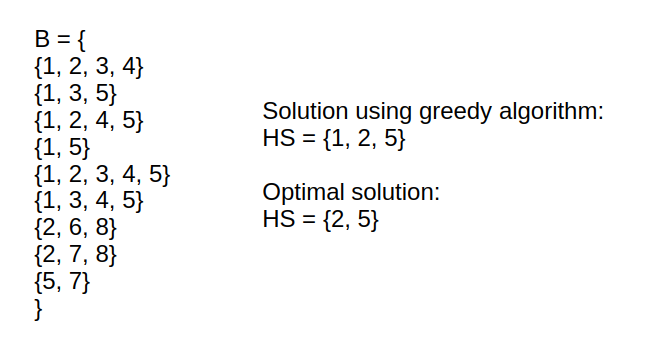
\includegraphics[width=0.9\textwidth]{img/greedyCmp.png}
\end{figure}